\section{Sensoren}
\begin{figure}[H]
	\ffigbox[\textwidth][]{%
		\begin{subfloatrow}
			\ffigbox[\FBwidth][]
			{\caption{Ultraschallsensor}}
			{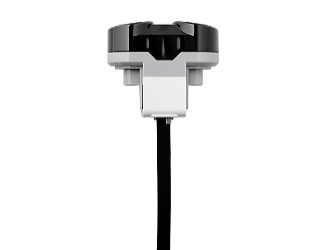
\includegraphics[]{images/ultrasonic.jpg}}
			\ffigbox[\FBwidth][]
			{\caption{Farbsensor}}
			{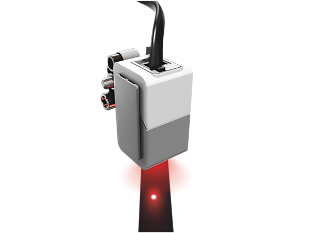
\includegraphics[]{images/color.png}}
		\end{subfloatrow}%\hspace*{\columnsep}%
		\begin{subfloatrow}
			\ffigbox[\FBwidth][]
			{\caption{Winkelsensor}}
			{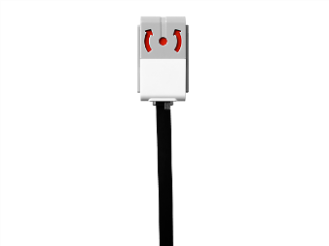
\includegraphics[]{images/gyro.png}}
			\ffigbox[\FBwidth][]
			{\caption{Ber"uhrungssensor}}
			{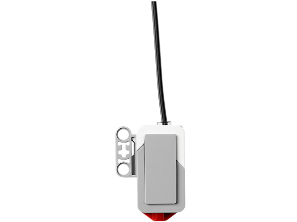
\includegraphics[]{images/touch.png}}
		\end{subfloatrow}
	}{}
\end{figure}

\begin{table}[h]
	\begin{tabular}{|p{0.2\textwidth}| p{0.7\textwidth}|}
		\hline
		Sensorausgang & lejos.hardware.port.SensorPort\\ \hline
		Ultraschallsensor& lejos.hardware.sensor.EV3UltrasonicSensor
		\\ \hline 
		Farbsensor & lejos.hardware.sensor.EV3ColorSensor\\ \hline 
		Winkelsensor & lejos.hardware.sensor.EV3GyroSensor\\ \hline 
		Ber"uhrungssensor & lejos.hardware.sensor.EV3TouchSensor\\ \hline 
	\end{tabular}
	\caption{ben"otigte Imports}
\end{table}

\begin{table}[H]
	\begin{tabular}{|p{0.2\textwidth}| p{0.7\textwidth}|}
		\hline
		setCurrentMode\newline (String mode)& setzt den Modus des Sensors \\ \hline 
		sampleSize() &  gibt die Anzahl der zur"uckgegeben Werte zurück\\ \hline 
		fetchsample(float[] signal, int offset) & Sensor misst und speichert es im Array \textbf{signal} ab Stelle \textbf{offset}\\ \hline
		getColorID() &  Farbsensor gibt erkannte Farbe zur"uck (-1=keine Farbe, 0=Rot, 1=Gr"un, 2=Blau, 3=Gelb, 6=Wei\ss{}, 7=Schwarz, 13=Braun)\\ \hline 
	\end{tabular}
	\caption{wichtige Methoden}
\end{table}

\begin{table}[H]
	\begin{tabular}{|p{0.2\textwidth}| p{0.7\textwidth}|}
		\hline
		Ultraschallsensor& Distance (Sensor gibt Distanz in Metern zur"uck) \\ \hline 
		Farbsensor &  Ambient (Sensor gibt Umgebungshelligkeit in Werten zwischen 0 und 1 zur"uck)\\ \hline 
		Winkelsensor& (Sensor gibt Winkel zur"uck)\\ \hline
		Ber"uhrungssensor& (Sensor gibt zur"uck, ob Taste gedr"uckt (1) oder nicht gedr"uckt (0) ist)\\ \hline
	\end{tabular}
	\caption{Modi}
\end{table}

Die Benutzung der Sensoren ist auf den ersten Blick etwas kompliziert, jedoch folgt die Benutzung einem festen Aufbau.\\

Zuerst muss wie bei den Motoren der Sensor benannt werden.\newline
\textbf{Bsp.: EV3UltrasonicSensor ultra = new EV3UltrasonicSensor(SensorPort.S1)}\\ \\
Als n"achstes muss der Sensor in den richtigen Modus gesetzt werden mit \newline \textbf{sensorname.setCurrentMode(String mode)}\\
\textbf{Bsp.: ultra.setCurrentMode(\glqq Distance\grqq{});}
\\ \\
Der n"achste Schritt ist das Anlegen eines Arrays, in dem die Daten gespeichert werden. Hierbei wird direkt mit \textbf{sampleSize()} die Gr"o\ss{}e gesetzt.
\textbf{Bsp.: float[] signal = new float[sensorname.sampleSize()];}
\\ \\
Um neue Daten zu erfassen wird mit dem Sensor die Methode \textbf{fetchSample} aufgerufen und im vorher angelegten Array gespeichert.\\
\textbf{Bsp.: ultra.fetchSample(signal, 0);}

